\documentclass[10pt]{article}
\topmargin=0.0in %length of margin at the top of the page (1 inch added by default)
\oddsidemargin=0.0in %length of margin on sides for odd pages
\evensidemargin=0in %length of margin on sides for even pages
\textwidth=6.5in %How wide you want your text to be
\marginparwidth=0.5in
\headheight=0pt %1in margins at top and bottom (1 inch is added to this value by default)
\headsep=0pt %Increase to increase white space in between headers and the top of the page
\textheight=9.1in %How tall the text body is allowed to be on each page

\usepackage{url}
\usepackage{graphicx}
\usepackage{authblk}
\usepackage{wrapfig}
\usepackage{draftwatermark}
\SetWatermarkText{DRAFT}
\SetWatermarkScale{5}

\renewcommand\Authfont{\fontsize{12}{14.4}\selectfont}
\renewcommand\Affilfont{\fontsize{9}{10.8}\selectfont}

\widowpenalty=500
\clubpenalty=500
\setlength{\parskip}{3pt}

\date{}

\begin{document}

\title{\textbf{Executive Summary}\\ADAM: Genomics Formats and Processing Patterns for Cloud Scale Computing}
\author[1]{Matt~Massie}
\author[1]{Frank~Austin~Nothaft}
\author[1,2]{Chris~Hartl}
\author[1]{Christos~Kozanitis}
\author[3]{Andr\'{e}~Schumacher}
\author[1]{Anthony~D.~Joseph}
\author[1]{David~Patterson}
\affil[1]{Department of Electrical Engineering and Computer Science, University of California, Berkeley}
\affil[2]{The Broad Institute of MIT and Harvard}
\affil[3]{International Computer Science Institute (ICSI), University of California, Berkeley}

\maketitle

\section{Introduction}

The overall volume of genomic data is rapidly increasing, thanks to a significant drop in sequencing costs~\cite{nhgri}.
Current genomics data formats and processing pipelines are not designed to scale well to large datasets. The current
Sequence/Binary Alignment/Map~(SAM/BAM) formats were intended for single node processing~\cite{li09}--- there have been
attempts to adapt BAM to distributed computing environments, but they see limited scalability past 8 nodes~\cite{niemenmaa12}. 
Additionally, due to the lack of an explicit data schema, there are well known incompatibilities between libraries that implement
SAM/BAM/Variant Call Format~(VCF) data access.

To address these problems, we introduce ADAM, a set of formats and processing stage implementations for genomic data.
ADAM is fully open source under the Apache 2 license, and is implemented on top of Avro and Parquet~\cite{avro, parquet}
for data storage. Our reference pipeline is implemented on top of Spark, a high performance in-memory map-reduce
system~\cite{zaharia10}. This provides the following advantages:

\begin{itemize}
\item Avro provides explicit data schema access in C/C++/C\#, Java/Scala, Python, php, and Ruby
\item Parquet allows access by database systems like Impala and Shark
\item Spark improves performance through in-memory caching and reduces I/O
\end{itemize}

In addition to improving the format's cross-platform portability, these changes lead to significant performance improvements. On a single
node, we are able to improve sort and duplicate marking performance by 2$\times$. On a 250 Gigabyte~(GB) high~(60$\times$) coverage
human genome, this system achieves a 53$\times$ speedup on a 100 node computing cluster.

\section{ADAM Data Format}

The ADAM format provides explicit schemas for read and reference oriented~(pileup) sequence data, variants, and genotypes. As explained
in the introduction, the schemas are implemented in Apache Avro, which is a cross-platform/language serialization format. Avro eliminates
the need for the development of language-specific libraries for format decoding/encoding, which eliminates the possibility of library
incompatibilities.

A key feature of ADAM is that any application that implements the ADAM schema is compatible with ADAM. This is important, as it prevents
applications from being locked into a specific tool or pattern. We envision that ADAM enables the stack shown in Figure 1. This stack is
inspired by the ``narrow waist'' of the Internet Protocol~(IP) suite.

\begin{wrapfigure}[18]{R}{0.25\textwidth}
  \begin{center}
    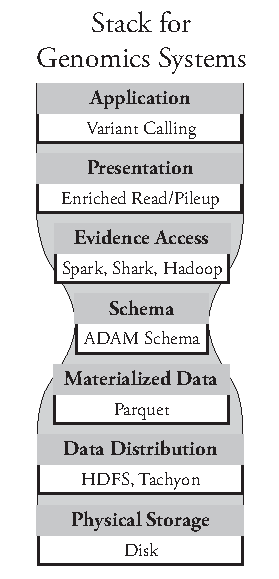
\includegraphics[width=0.25\textwidth, trim=0 30 0 15]{stack-model.pdf}
  \end{center}
  \caption{Stack Model}
\end{wrapfigure}

In addition to the advantages outlined above, ADAM eliminates the file headers in modern genomics formats. All header information is available
inside of each individual record. The variant and genotype formats also demonstrate two significant improvements. First, these formats are
co-designed so that variant data can be seamlessly calculated from a given collection of sample genotypes. Secondly, these formats are designed
to flexibly accommodate annotations without cluttering the core variant/genotype schema. In addition to the benefits described above, ADAM
files are 25\% smaller on disk than compressed BAM files.

\section{Pipeline Construction and Performance}

The ADAM processing pipeline uses Spark as a compute engine and Parquet for data access. Spark is an in-memory MapReduce framework
which minimizes I/O accesses. We chose Parquet for data storage as it is an open-source columnar store that is designed for distribution across
multiple computers with high compression. Additionally, Parquet supports efficient methods~(predicates and projections) for accessing only a
specific segment or fields of a file, which can provide significant~(2-10$\times$) speedups for genomics data access patterns.

At this date, we have implemented Sort and Duplicate Marking in the ADAM pipeline. BQSR and Indel Realignment implementations are
forthcoming. The performance of these stages is shown in Table 1.

\begin{table}[h]
\small
\caption{Sort (L) and Duplicate Marking (R) for NA12878}
\begin{center}
\begin{tabular}{| l | c | c |}
\hline
\bf Software & \bf EC2 profile & \bf Wall Clock Time \\
\hline
\hline
Picard 1.103 & 1 \texttt{hs1.8xlarge} & 17h 44m \\
ADAM 0.5.0 & 1 \texttt{hs1.8xlarge} & 8h 56m \\
ADAM 0.5.0 & 32 \texttt{cr1.8xlarge} & 33m \\
ADAM 0.5.0 & 100 \texttt{m2.4xlarge} & 21m \\ 
\hline
\end{tabular}
\begin{tabular}{| l | c | c |}
\hline
\bf Software & \bf EC2 profile & \bf Wall Clock Time \\
\hline
\hline
Picard 1.103 & 1 \texttt{hs1.8xlarge} & 20h 22m \\
ADAM 0.5.0 & 100 \texttt{m2.4xlarge} & 29m \\
\hline
\end{tabular}
\end{center}
\end{table}

\noindent These tests were run on a high coverage~(60$\times$) full genome sequencing of NA12878.

\section{Conclusion}

This executive summary and the attached technical report introduce ADAM, a data format that is optimized for high performance
distributed genomic data processing pipelines. ADAM is a modular system that is open source under the Apache 2 license. On
traditional workloads, ADAM provides a $>$50$\times$ speedup, and ADAM files are 25\% smaller than their compressed BAM
equivalents.

\footnotesize

\bibliographystyle{acm}

\bibliography{adam-tr-executive}

\end{document}
